\chapter{Extraktion raumakustischer Parameter}
\section{Die Nachhallzeit $\mathbf{RT_{60}}$}
\label{sec:rt60}Wir analysieren die Impulsantwort des Raumes HFT616 der TU Berlin.
Das Signal hat eine Abtastrate von $f_s$ = 44100 Hz und enthält am Anfang einen Bereich mit Grundrauschen bevor die eigentliche Impulsantwort beginnt.
Als erstes entfernen wir diesen Teil des Signals.
Als Kriterium zur Bestimmung des zeitlichen Nullpunkts der Impulsantwort verwenden die Position des ersten lokalen Maximums vor dem absoluten Maximum .
Zur Bestimmung der Nachhallzeit der gegebenen Impulsantwort haben wir die Schroeder Methode \cite{Schroeder65} verwendet.
Dazu haben wir in Matlab folgende Gleichung implementiert:

\begin{align*}
R[n] = \sum_{i=1}^N h^2[i] + \sum_{i=1}^n h^2[i]
\end{align*}
Aus diesem Vektor lässt sich wiederum eine diskretisierte Form der Energy Decay Curve berechnen, welche den auf 0 dB normierten Pegelabfall des Signals  beschreibt:
\begin{align*}
EDC_{norm}[n] = 10 \cdot \mathrm{log}_{10} \left(\frac{R[n]}{\sum_{i=1}^N h^2[i]}\right)
\end{align*}
Um daraus nun einen Wert für die Nachhallzeit T$_{60}$ zu bestimmen, haben wir T$_{20}$ und T$_{30}$ berechnet.
Dabei haben wir zunächst Indexdifferenzen gebildet und diese dann in Zeitwerte umgerechnet.
Für T$_{20}$ haben wir die Punkte die Pegelabfällen zwischen -5 dB und -25 dB in $EDC_{norm}[n]$ entsprechen verwendet, für T$_{30}$, die Differenz zwischen den -5 dB und -35 dB Punkten.
Dieses Vorgehen entspricht der DIN Norm .......? .
Als Ergebnis für die Nachhallzeit bekommen wir T$_{60,1}$ = 0,86 s, wenn wir sie aus T$_{30}$ berechnen und T$_{60,2}$ = 0,79 s, wenn wir T$_{20}$ verwenden.




\begin{figure}[H]
    \center
    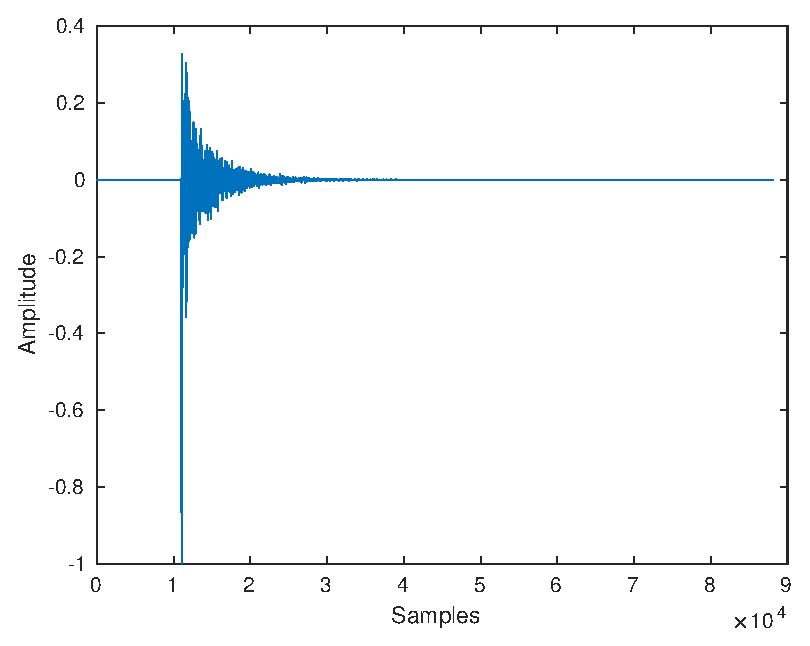
\includegraphics[width = 0.7\textwidth]{figures/samples}
    \caption{Die Impulsantwort}
    \label{fig:im}
\end{figure}

\begin{figure}[H]
    \center
    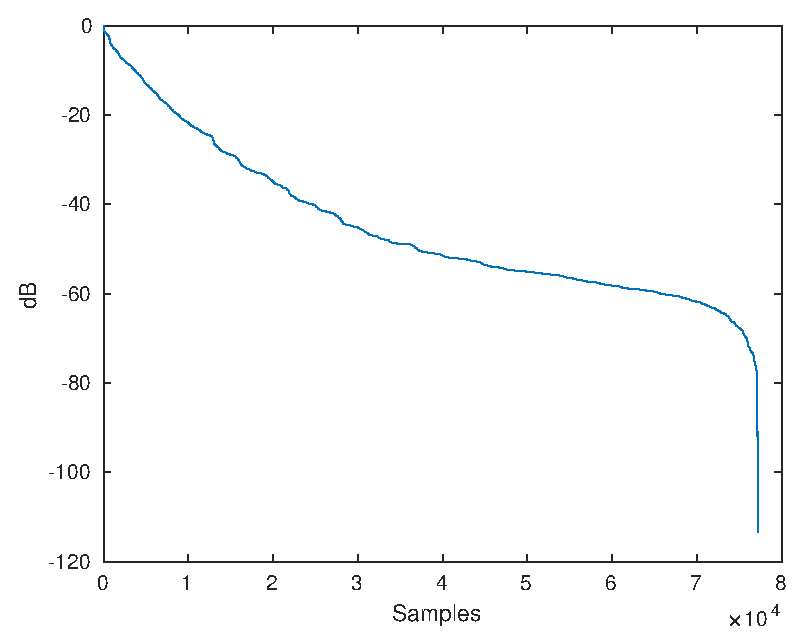
\includegraphics[width = 0.7\textwidth]{figures/EDC_norm.eps}
    \caption{EDC norm}
    \label{fig:edc}
\end{figure}

\section{Das Bassverhältnis $\mathbf{BR}$}
\label{sec:br}
Um das Bassverhältnis zu bestimmen ermitteln wir die Nachhallzeiten in verschiedenen Frequenzbereichen. Dazu filtern wir die Impulsantwort in Oktavbändern.
Wir generieren also vier neue Signale mittels Butterworth-Filtern dritter Ordnung mit Mittenfrequenzen bei 125 Hz, 250 Hz, 500 Hz und 1000 Hz. Auf diese wenden wir dieselbe Routine, wie in Aufgabe A) an, beschränken uns aber auf die Berechnung mittels $T_20$, um daraus die Nachhallzeiten $T_{125 \mathrm{Hz}}$ = 0,94 s, $T_{250 \mathrm{Hz}}$ = 0,63 s, $T_{500 \mathrm{Hz}}$ = 0,67 s und $T_{1000 \mathrm{Hz}}$ = 0,61 s zu erhalten.
Für das Bassverhältnis BR folgt somit:
\begin{align*}
BR = \frac{T_{125 \mathrm{Hz}} + T_{250 \mathrm{Hz}}}{T_{500 \mathrm{Hz}} + T_{1000 \mathrm{Hz}}} = 1,23
\end{align*}  
Laut dem Handbuch der Audiotechnik (Lit.verweis!!) wird solch ein Wert bei Musikaufführungsräumen angestrebt, in welchen der $BR$-Wert zwischen 1.0 und 1.3 liegen sollte.
Für Sprache hingegen sollte der Wert unterhalb von 1.0 liegen.

\section{Das Klarheitsmaß $\mathbf{C_{80}}$}
\label{sec:c80}
Für dieselben oktavbandgefilterten Signale, wie in Aufgabenteil B) können wir nun das Klarheitsmaß $C_{80}$ für die vier Frequenzbänder bestimmen.
Dieses kann durch folgende wiederum diskretisierte Formel berechnet werden
\begin{align*}
C_{80} = 10\cdot \mathrm{log}_{10}\left(\frac{ \sum_{i=1}^{n_{80}} h^2[i]}{\sum_{i=n_{80}}^N h^2[i]}\right)
\end{align*}
wobei $n_{80} = 80 \mathrm{ms} \cdot f_s$ gilt. \\
Als Ergebnisse erhalten wir folgende Werte:
\begin{table}[H]
\centering
\begin{tabular}{ c | c }
  Frequenzband & $C_{80}$ \\
  \hline
  125 Hz & 2,91 \\
  250 Hz & 7,75 \\
  500 Hz & 8,23 \\
  1000 Hz & 8,63  \\
  \end{tabular}
\end{table}

Interpretation der Werte????

\section{Der interaurale Kreuzkorrelationkoeffizient $\mathbf{IACC}$}
\label{sec:iacc}

Der interaurale Kreuzkorrelationskoeffizient gibt Auskunft über zeitliche Unterschiede des an beiden Ohren ankommenden Schalls und somit über die "Räumlichkeit" des Klangeindrucks in einem Raum. 
Für die Berechnung dieses Maßes benötigen wir eine binaurale Impulsantwort, also ein an zwei verschiedenen Stellen im Abstand der menschlichen Ohren aufgenommenes Signal. 
Es wird berechnet, bei welchen Zeitdifferenzen $\tau$ die beiden Signale für linkes und rechtes Ohr maximal korrelieren.
Dabei werden lediglich $\tau$-Werte aus dem Bereich zwischen -1 ms und 1 ms betrachtet, was den Bereich einschließt, den Schall braucht um vom einen zum anderen Ohr zu gelangen.  
Desweiteren unterscheidet man zwischen $IACC_{\mathrm{early}}$ und $IACC_{\mathrm{late}}$, je nachdem welcher Teil der Impulsantwort analysiert wird. Wie im Handbuch der Audiotechnik (Lit.verweis!!) empfohlen verwenden wir für den frühen interauralen Kreuzkorrelationskoeffizienten das Zeitintervall zwischen $t_1$ = 0 ms und $t_2$ = 80 ms und für den späten Koeffizienten den Bereich zwischen 80 ms und 1000 ms. 
Die in Matlab implementierte diskretisierte Gleichung lautet:
\begin{align*}
IACC = \mathrm{max}\left( \frac{\sum_{i=n_1}^{n_2} p_L(i)p_R(i+\Delta n)} {\sqrt{\sum_{i=n_1}^{n_2}p_R(i)^2 \sum_{i=n_1}^{n_2} p_R(i)^2 }})\right) 
\end{align*}
Hierbei gilt $n_1 = t_1 \cdot f_s$,  $n_2 = t_2 \cdot f_s$ sowie $\Delta n = \tau \cdot f_s$.
Wir haben die Koeffizienten abermals für die vier Oktavbänder berechnet.
Die Ergebnisse sind in folgender Tabelle aufgelistet:
\begin{table}[H]
    \centering
    \caption{Die Werte für $IACC_{Early}$ und $IACC_{Late}$}
    \label{tab:iacc}
    \begin{tabular}[\textwidth]{|l|l|l|}
        \hline
        Oktavbänder & Early & Late \\
        \hline
        125 & 0.9890 & 0.9355 \\
        \hline
        250 & 0.8986 & 0.7937 \\
        \hline
        500 & 0.2102 & 0.1034 \\
        \hline
        1000 & 0.4616 & 0.1902 \\
        \hline
    \end{tabular}
\end{table}

\section{Absorptionsgrad der Wandfläche $\mathbf{\alpha_{80}}$}
\label{sec:alpha}

\begin{table}[H]
    \centering
    \caption{Der Absorptionsgrad $\alpha$ für die verschiedenen Bänder}
    \label{tab:alpha}
    \begin{tabular}[\textwidth]{|l|l|l|}
        \hline
        Oktavbänder &  $\alpha$\\
        \hline
        125 & 0.1346 \\
        \hline
        250 & 0.2014 \\
        \hline
        500 & 0.1898 \\
        \hline
        1000 & 0.2085 \\
        \hline
        Durchschnitt & 0.1836 \\
        \hline
    \end{tabular}
\end{table}


\section{Vergleich der Nachhallzeiten}
\label{sec:ts}


\section{Die Schalldruckpegelverteilung}
\label{sec:sdpv}